% Created 2024-07-08 Mon 22:16
% Intended LaTeX compiler: pdflatex
\documentclass[11pt]{article}
\usepackage[utf8]{inputenc}
\usepackage[T1]{fontenc}
\usepackage{ragged2e}
\usepackage{caladea}
\usepackage{graphicx}
\usepackage{longtable}
\usepackage{wrapfig}
\usepackage{rotating}
\usepackage{epigraph}
\usepackage[normalem]{ulem}
\usepackage{hyperref}
\usepackage{amsmath}
\usepackage{amssymb}
\usepackage{capt-of}
\usepackage{hyperref}
\usepackage{fancyhdr}
\title{Novena à Santa Bibiana}
 % \hypersetup{
 %  pdfauthor={},
 %  pdftitle={Novena a/à SANTO_NOME},
 %  pdfkeywords={},
 %  pdfsubject={},
 %  pdfcreator={Emacs 29.4 (Org mode 9.6.15)}, 
 %  pdflang={English}
 % }

\title{
  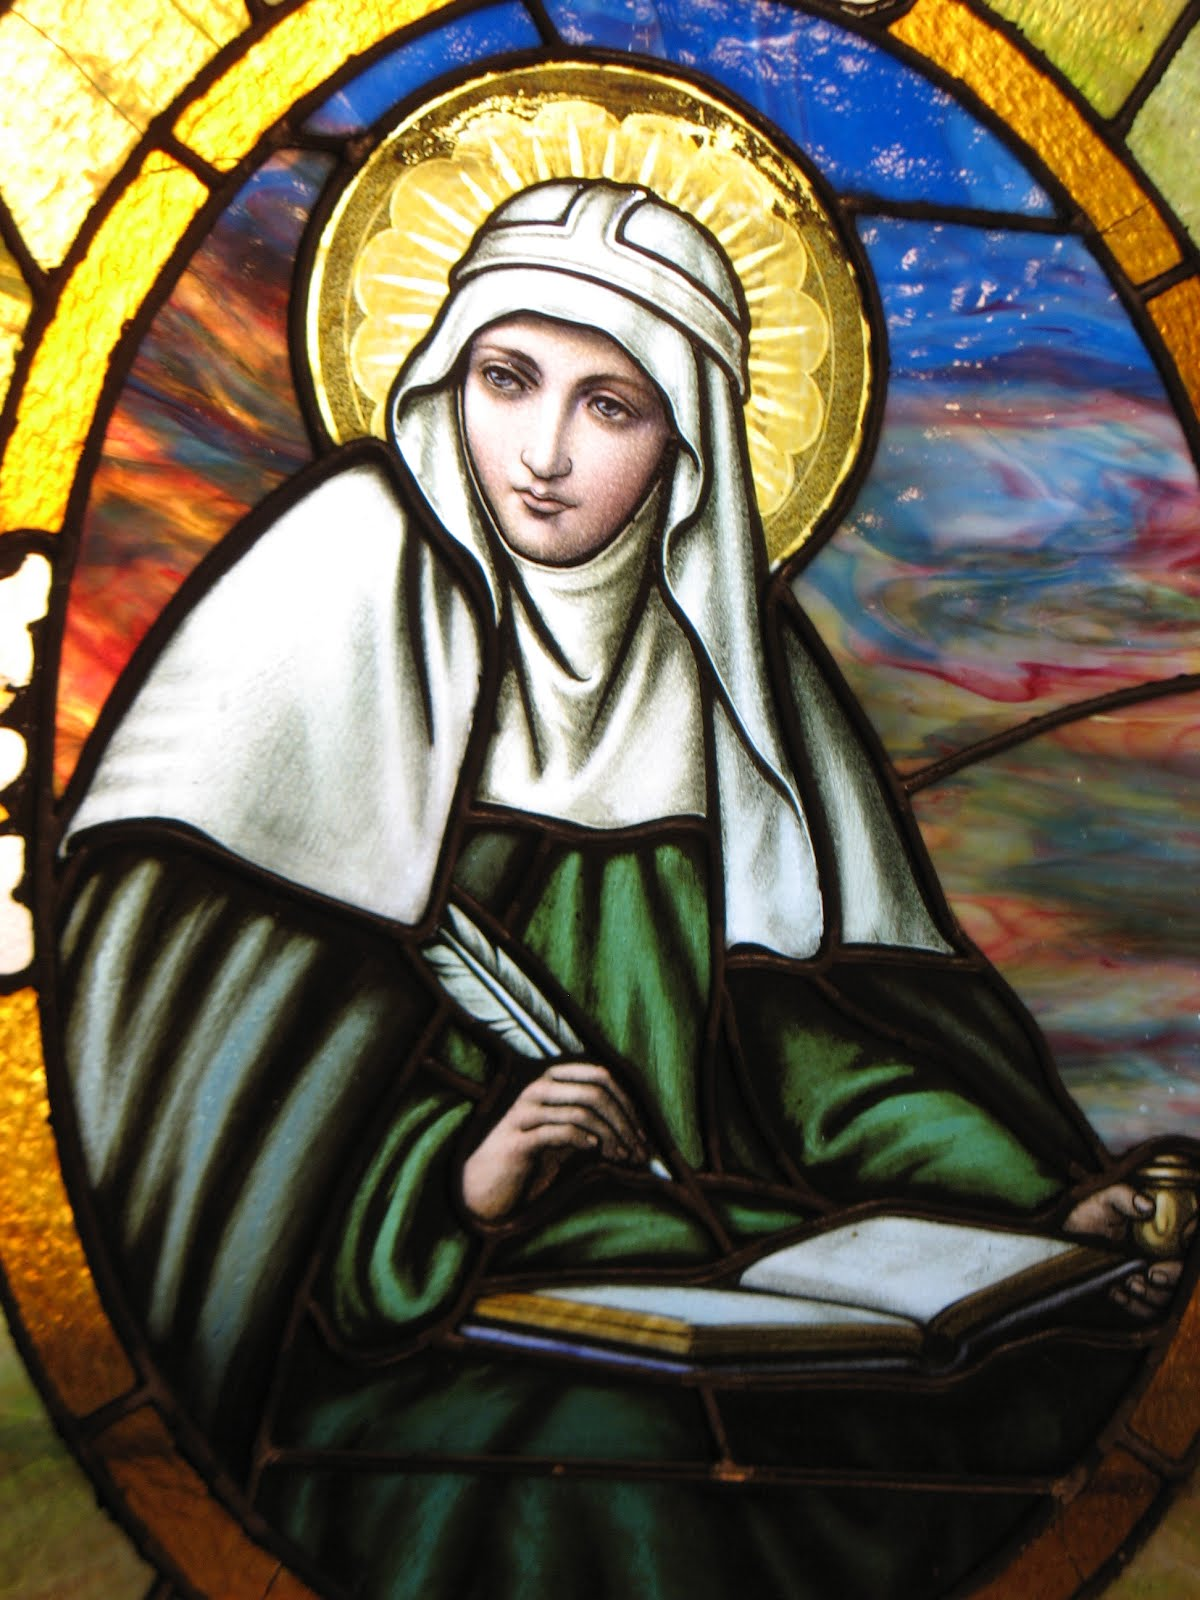
\includegraphics[scale=0.28]{./assets/imagem.jpg}
  \par
   Quinze Orações de Santa Brígida}
\author{}
\date{}
\renewcommand{\contentsname}{Sumário}

\begin{document}
\maketitle

\thispagestyle{empty}

\pagestyle{fancy}
\fancyhf{} % clear existing header/footer entries
\fancyfoot[LO, CE]{
  
\includegraphics[scale=0.2]{./assets/cross.png}}

% Place Page X of Y on the right-hand
% side of the footer
\fancyfoot[R]{\thepage}
  
\newpage

\tableofcontents

\centering
\vfill
Visite-nos no Telegram: \url{https://t.me/CotidieNovena}
\newpage


\section{História}
\subsection{Santa Brígida da Suécia}
\begin{justify}
Santa Brígida, conhecida por suas profundas experiências místicas e ardente devoção a Deus, é uma figura inspiradora para todos os cristãos. Nasceu na Suécia no século XIV e fundou a Ordem do Santíssimo Salvador, dedicando sua vida à oração, ao serviço e à busca de uma união íntima com o Senhor. Suas revelações celestiais e visões de Cristo a tornaram uma conselheira espiritual respeitada, cujo exemplo de fé e humildade continua a tocar os corações dos fiéis. Ao nos dirigirmos a Santa Brígida em oração, buscamos sua intercessão para fortalecer nossa própria fé e espiritualidade. Pedimos sua ajuda para encontrar a paz e a presença de Deus em nossas vidas diárias, seguindo seus passos de amor, serviço e devoção.

\begin{center}
 \subsection{A devoção das Quinze Orações}
\end{center}


As quinze orações a seguir, atribuídas a S. Brígida da Suécia (1303-1373), muito provavelmente foram escritas por místicos da sua Ordem, no século XV. Foram publicadas inúmeras vezes ao longo dos séculos, com variação considerável nos textos e até mesmo na ordem das invocações.

Constituem, em si mesmas, \textbf{uma meditação piedosa sobre os mistérios da Paixão e Morte de Cristo.} Eram bastante populares durante a Baixa Idade Média, sendo item frequente nos manuais de oração da época. Cumprem um duplo propósito: catequético, instruindo as pessoas nos episódios mais importantes da vida de Nosso Senhor, e penitencial, excitando-lhes o amor a Deus e o arrependimento dos próprios pecados.

\textbf{Em muitos lugares estas preces estão associadas a uma lista de promessas} supostamente reveladas a S. Brígida quando de sua visita à Basílica de São Paulo Fora dos Muros, em Roma. As tais promessas listam uma série de incríveis benefícios, que seriam concedidos a quem recitasse estas orações todos os dias ao longo de um ano, e incluem a libertação de 15 almas dos entes queridos do Purgatório e a conversão de 15 pecadores da própria família. A verdade, porém, é \textbf{que essas promessas jamais foram feitas a S. Brígida e tampouco têm qualquer aprovação eclesiástica que seja.}

É muito de se lamentar que essas promessas ainda constem em livros de oração nos nossos dias, pois a própria Congregação do Santo Ofício proibiu, em 1954, a sua publicação [1]. Mas, ainda que não houvesse uma censura a essas promessas vinda de Roma, o conteúdo delas é, de fato, arbitrário e fantástico demais para ser credível. Não temos dúvidas de que \textbf{abundantes frutos espirituais podem ser colhidos da leitura e meditação das linhas abaixo,} mas promessas como as que circulam, associadas a estas orações, terminam transformando em superstição o que deveria ser antes um convite ao fervor na oração, à conversão interior e ao apostolado com as pessoas mais próximas de nós.

\hfill

\subsubsection*{Observações:}
\begin{enumerate}
 \item O "Terço" de Santa Brígida é, na verdade, uma série de orações e meditações. Não é um “terço” no sentido tradicional, mas é frequentemente referido como tal devido à sua estrutura repetitiva."
 \item A tradução abaixo foi feita pela Equipe Cristo Nihil Pr\ae ponere a partir do texto em latim encontrado na edição de 1670 do livro Paradisus Anim\ae\ Christian\ae\, de Jacob Merlo Horst, e que também pode ser acessado no site Preces Latinæ.
\end{enumerate}

\end{justify}

\hfill


\newpage

%%%%%%%%%%%%%%%%%%%%%%%%%%%%%%%%%%%%% Orações  %%%%%%%%%%%%%%%%%%%%%%%%%%%%%%%%%%%%%%%%%%%

\section{Orações}\label{sec:Orações} % (fold)

\subsection{Oração Inicial} % (fold)

“Meu Senhor, pelos Santos Inocentes, quero Vos rogar hoje por todos aqueles que são injustiçados, sofrem ameaças, são marginalizados e incompreendidos. Olhai pelos pequeninos, abandonados e assassinados pelas estruturas de morte de nossa sociedade. Que convosco eles alcancem dignidade e paz. Amém.”

\textbf{Pai Nosso, Avs Maria, Glória}

\subsection{Oração I.}
Ó Jesus Cristo, eterna doçura dos que vos amam, júbilo que excede toda alegria e todo desejo, salvação e amante dos pecadores, que achais vossas delícias em estar com os filhos dos homens e pelo homem vos fizestes homem na plenitude dos tempos: lembrai-vos de tudo o que previstes e da íntima tristeza que, em vosso Corpo humano, suportastes ao aproximar-se o tempo de vossa salubérrima Paixão, preordenado em vosso divino Coração.

Lembrai-vos da tristeza e da amargura que, pelo vosso testemunho, tivestes em vossa Alma, quando, na Última Ceia, entregastes aos vossos discípulos o vosso Corpo e Sangue, lavastes-lhes os pés e, consolando-os docemente, predissestes vossa iminente Paixão. 

Lembrai-vos de todo o tremor, da angústia e da dor que em vosso delicado Corpo, antes da Paixão de vossa Cruz, suportastes quando, após vossa tríplice oração e o suor de Sangue, fostes traído por Judas, vosso discípulo; preso pela gente escolhida; acusado por falsas testemunhas; injustamente julgado por três juízes; condenado, embora inocente, na cidade eleita, no tempo pascal, na florida juventude de vosso Corpo; despido da vossa própria veste e coberto de vestes alheias; esbofeteado; tivestes vossos olhos e rosto cobertos e fostes espancado, preso à coluna, flagelado, coroado de espinhos, com uma cana ferido na cabeça e lacerado com inumeráveis outras calúnias.

Dai-me, Senhor Deus, eu vo-lo peço, pela memória dessas paixões antes de vossa Cruz, uma verdadeira contrição antes de minha morte, uma pura Confissão, uma digna satisfação e a remissão de todos os pecados. Amém. 

\textbf{Pai-Nosso, Ave-Maria, Glória.}

\subsection{Oração II.}
Ó Jesus, criador do mundo, a quem nenhuma dimensão pode compreender, que abarcais a Terra com um palmo: recordai-vos de vossa amaríssima dor, que suportastes quando os judeus pregaram vossas santíssimas mãos à Cruz com pregos embotados e, a fim de perfurar vossos delicadíssimos pés, como não lhes fosse o bastante, acrescentaram dor sobre dor às vossas chagas, e assim cruelmente vos distenderam e estenderam pelos braços de vossa Cruz, para que se dissolvessem os vínculos dos vossos membros.

Eu vos imploro, pela memória desta sacratíssima e amaríssima dor na Cruz, que me deis o vosso temor e amor. Amém. 

\textbf{Pai-Nosso, Ave-Maria, Glória.}

\subsection{Oração III.}
Ó Jesus, médico celeste, recordai-vos do langor, do livor e da dor que, elevado no alto patíbulo da Cruz, padecestes em todos os vossos membros dilacerados, dos quais nenhum permaneceu em bom estado, de modo que não se achasse dor nenhuma semelhante à vossa, pois desde a planta dos pés até o alto da cabeça não havia em vós coisa sã, e no entanto, esquecido de todas as dores, rogastes piedosamente ao Pai pelos vossos inimigos, dizendo: “Pai, perdoa-lhes, porque não sabem o que fazem”. Por esta misericórdia e pela memória daquela dor, concedei-me que esta memória de vossa amaríssima Paixão me alcance a plena remissão de todos os meus pecados. Amém. 

\textbf{Pai-Nosso, Ave-Maria, Glória.}

\subsection{Oração IV.}
Ó Jesus, verdadeira liberdade dos anjos, paraíso de delícias, lembrai-vos da tristeza e do horror que suportastes, quando todos os vossos inimigos, quais leões ferocíssimos, puseram-se ao vosso redor e, com bofetadas, cusparadas, lacerações e outras penas inauditas, vos maltrataram.

Por estas penas e por todas as palavras contumeliosas e os duríssimos tormentos com que vos afligiram, Senhor Jesus Cristo, todos os vossos inimigos, eu vos imploro que me livreis de todos os meus inimigos, visíveis e invisíveis, e me deis chegar, à sombra de vossas asas, à perfeição da salvação eterna. Amém. 

\textbf{Pai-Nosso, Ave-Maria, Glória.}

\subsection{Oração V.}
Ó Jesus, espelho da claridade eterna, lembrai-vos daquela tristeza que tivestes quando, no espelho de vossa sereníssima majestade, vistes a predestinação dos eleitos, que se haviam de salvar pelos méritos de vossa Paixão, e a reprovação dos maus, que pelos seus deméritos se haviam de condenar, e pelo abismo de vossa piedade, com que vos compadecestes de nós, pecadores e desesperados, e que manifestastes ao ladrão na Cruz, dizendo: “Hoje estarás comigo no paraíso”, rogo-vos, piedoso Jesus, que tenhais misericórdia de mim na hora de minha morte. Amém. 

\textbf{Pai-Nosso, Ave-Maria, Glória.}

\subsection{Oração VI.}
Ó Rei amável e amigo todo desejável, lembrai-vos daquela tristeza que tivestes quando, nu e miserável, pendestes na Cruz, e todos os vossos amigos e conhecidos se voltaram contra vós, e não encontrastes ninguém que vos consolasse, além de vossa dileta Mãe, de pé na amargura de sua alma fidelíssima a vós, que confiastes ao vosso discípulo, dizendo: “Mulher, eis aí o teu filho”.

Rogo-vos, piíssimo Jesus, pela espada de dor que transpassou a alma dela, que vos compadeçais de mim em todas as minhas tribulações e aflições, corporais e espirituais, e dai-me a consolação no tempo da tribulação e na hora de minha morte. Amém. 

“Queda no Caminho do Calvário”, de Rafael.

\textbf{Pai-Nosso, Ave-Maria, Glória.}

\subsection{Oração VII.}
Ó Jesus, fonte de inexaurível piedade, que por um íntimo afeto de amor dissestes na Cruz: “Tenho sede”, isto é, da salvação do gênero humano, acendei, vo-lo peço, em nossos corações o desejo de perfeição, e abrandai e extingui de todo em nós a sede da concupiscência e o ardor dos prazeres mundanos. Amém. 

\textbf{Pai-Nosso, Ave-Maria, Glória.}

\subsection{Oração VIII.}
Ó Jesus, doçura dos corações e poderosa suavidade das mentes, pelo azedume do vinagre e do fel que por nós provastes, concedei-nos, na hora de nossa morte, receber dignamente o vosso Corpo e Sangue, como remédio e consolação para nossas almas. Amém. 

\textbf{Pai-Nosso, Ave-Maria, Glória.}

\subsection{Oração IX.}
Ó Jesus, virtude régia, júbilo espiritual, lembrai-vos da angústia e da dor que padecestes quando, pelo amargor da morte e os insultos dos judeus, com alta voz clamastes, abandonado por Deus Pai: “Meu Deus, meu Deus, por que me abandonastes?” Por esta angústia vos peço que nas nossas angústias não nos abandoneis, Senhor Deus nosso. Amém. 

\textbf{Pai-Nosso, Ave-Maria, Glória.}

\subsection{Oração X.}
Ó Jesus, Alfa e Ômega, vida e poder em todo tempo, recordai-vos que desde o alto da cabeça até a planta do pé vos mergulhastes por nós na água da Paixão.

Pela largura e extensão de vossas chagas, ensinai-me a mim, afundado em muitos pecados, a guardar por verdadeira caridade a Lei que promulgastes. 

\textbf{Pai-Nosso, Ave-Maria, Glória.}

\subsection{Oração XI.}
Ó Jesus, abismo profundíssimo de misericórdia, rogo-vos, pela profundidade de vossas chagas, que atravessaram a medula de vossos ossos e vísceras, que me tireis da água de pecado em que estou submerso e me escondais, no interior de vossas chagas, do rosto de vossa ira, até que passe o vosso furor, Senhor. Amém. 

\textbf{Pai-Nosso, Ave-Maria, Glória.}

\subsection{Oração XII.}
Ó Jesus, espelho da verdade, sinal de unidade e vínculo de caridade, lembrai-vos da multidão de vossas chagas, com que, da cabeça aos pés, fostes vulnerado e rubricado com vosso santíssimo Sangue, multidão de dores que suportastes em vossa carne virginal por nós! Piedoso Jesus, que mais deveríeis fazer e não fizestes?

Gravai, vo-lo peço, ó piedoso Jesus, todas as vossas chagas no meu coração com o vosso preciosíssimo Sangue, para que nelas eu leia sempre a vossa dor e morte e persevere constante até o fim em ação de graças. Amém. 

\textbf{Pai-Nosso, Ave-Maria, Glória.}

\subsection{Oração XIII.}
Ó Jesus, leão fortíssimo, Rei imortal e invencível, lembrai-vos da dor que padecestes quando todas as forças do vosso Coração e Corpo de todo se acabaram e, reclinando a cabeça, dissestes: “Tudo está consumado”. 

Por esta angústia e dor, tende misericórdia de mim, quando minha alma, no momento do último suspiro, estiver vexada e conturbada. Amém. 

\textbf{Pai-Nosso, Ave-Maria, Glória.}

\subsection{Oração XIV.}
Ó Jesus, unigênito do altíssimo Pai, esplendor e figura de sua substância, lembrai-vos da esforçada entrega com que entregastes o espírito ao Pai, dizendo: “Pai, em tuas mãos entrego o meu espírito” e, de Corpo lacerado, de Coração alquebrado, com grande clamor, abertas as vísceras de vossa misericórdia para nos redimir, expirastes.

Por esta preciosíssima morte vos imploro, Rei dos santos, que me fortaleçais para resistir ao diabo, ao mundo, à carne e ao sangue, a fim de que, morto(a) para o mundo, eu viva para vós, e na hora suprema de minha partida acolhei-me o espírito degredado e peregrino a retornar para vós. Amém. 

\textbf{Pai-Nosso, Ave-Maria, Glória.}

\subsection{Oração XV.}
Ó Jesus, videira verdadeira e fecunda, lembrai-vos da abundante efusão do vosso Sangue, que vós, qual sumo arrancado ao cacho, copiosamente derramastes quando, na cruz, calcastes sozinho o lagar, e do vosso lado aberto pela lança do soldado nos propinastes Sangue e água, de modo que nem uma só gota permanecesse em vós; e quando, enfim, fostes suspenso no alto, qual um feixe de mirra, e vossa carne delicada se desfez, e o licor de vossas vísceras se secou, e a medula de vossos ossos murchou. 

Por esta vossa amaríssima Paixão e pela efusão do precioso Sangue, piedoso Jesus, imploro-vos que recebais minha alma na agonia de minha morte. Amém. 

\textbf{Pai-Nosso, Ave-Maria, Glória.}

\vfill
\subsection{Conclusão} Ó Senhor Jesus Cristo, Filho do Deus vivo, acolhei esta oração com aquele amor excelentíssimo com que suportastes todas as chagas do vosso santíssimo Corpo e tende misericórdia de mim, vosso servo, e dai a todos os pecadores e a todos os fiéis, tanto vivos quanto defuntos, misericórdia, graça, remissão e a vida eterna. Amém.

\subsection*{Créditos:}
\begin{itemize}
 \item \href{https://padrepauloricardo.org/blog/quinze-oracoes-em-honra-a-paixao-de-cristo}{Equipe Cristo Nihil Pr\ae ponere}
 \item \href{https://cruzterrasanta.com.br/oracao-terco-de-santa-brigida/399/105/}{Cruz Terra Santa}
\end{itemize}

\end{document}
